\documentclass[10pt]{scrartcl}

\usepackage[margin=3.0cm]{geometry}                % See geometry.pdf to learn the layout options. There are lots.
\geometry{letterpaper}                   % ... or a4paper or a5paper or ... 
%\geometry{landscape}                % Activate for for rotated page geometry
%\usepackage[parfill]{parskip}    % Activate to begin paragraphs with an empty line rather than an indent
\usepackage{graphicx}
\usepackage{amssymb}
\usepackage{amsmath}
\usepackage{epstopdf}
\usepackage{multirow}

\title{Ideal helix geometry}

\author{Ivana}
          
\begin{document}
\maketitle



\section{Overview}



\begin{figure}[h]\label{triangle}
\centering{\includegraphics[width=0.4\linewidth]{helix.png}}
\centering{\includegraphics[width=0.4\linewidth]{triangle.png}}
  \caption {Distance between $c_\alpha$1 and $c_\alpha$3.}
\end{figure}


$c$ is climb (=$1.5$\AA). The angle $\alpha = 100 \deg$. The radius of the helix, $r$, is 2.3\AA. 

Solving for $t_{13}$ (Fig.\, \ref{triangle}).
$t_{13}$  is the chord over the angle  $2\pi-2\alpha$:

\begin{equation}
t_{13} = 2r\sin\left(\frac{2\pi-2\alpha}{2}\right)
\end{equation}

Then the distance between $c_\alpha$1 and $c_\alpha$3:
\begin{equation}
d_{13} = (2c)^2+t_{13}^2 = 5.43\AA.
\end{equation}

Similarly
\begin{eqnarray}
t_{14} = 2r\sin\left(\frac{2\pi-3\alpha}{2}\right) \\
d_{14} = (3c)^2+t_{13}^2 = 5.05\AA.
\end{eqnarray}




\end{document}  
